\documentclass{scrreport}
\usepackage[ngerman]{babel}
\usepackage[utf8]{inputenc}
\usepackage[combine]{ucs}
\usepackage[pdftex]{graphicx}
\usepackage[final]{pdfpages}
\usepackage{listings} % source code formatting
\usepackage{blindtext}
\usepackage{wrapfig}
\usepackage{subfigure}
\usepackage{float}
\usepackage{subfiles}
\usepackage[numbers]{natbib}
\usepackage{fullpage}
\usepackage{hyperref}
\usepackage{courier}
\usepackage{color}
\usepackage{xcolor}
\usepackage{scrhack}
\usepackage{siunitx}
\usepackage{newfloat}
\DeclareFloatingEnvironment[
  fileext=lg,
  name=Code-Snippet,
  placement=htp,
]{code}
\bibliographystyle{unsrt}
\graphicspath{{images/}{../images/}} % set correct path to images
\headsep = 35pt

\DeclareOldFontCommand{\bf}{\normalfont\bfseries}{\mathbf}

\ifx\pdftexversion\undefined
\usepackage[dvips]{graphicx}
\else
\usepackage[pdftex]{graphicx}
\DeclareGraphicsRule{*}{mps}{*}{}
\fi

\setcounter{secnumdepth}{3}
\setlength{\parskip}{6pt plus0pt minus0pt}
\setlength{\parindent}{0pt}
\pagestyle{headings} 

\begin{document}
\begin{titlepage}
	\begin{center}
		\Large{Diplomarbeit} \\
		
		\bigskip
		\bigskip
		\bigskip

		\Huge{Elektromotoren im Unterricht} \\
		\bigskip
		\bigskip
		\bigskip
		\huge{Verständnis und arbeiten mit Gleichstrommotoren} \\

		\bigskip
		\bigskip
		\bigskip
		\large{erstellt von} \\

		\bigskip
		\bigskip
		\bigskip
		
		\Huge{Leonhard Erharter} \\
		\Huge{(Matteo Juen)} \\
		\bigskip
		\bigskip
		\bigskip

		
		\bigskip
	    \bigskip
        
        
\includegraphics[width=1cm]{../images/htl-logo}

		\Large{HTBLuVA} \\
		\Large{Innsbruck Anichstrasse} \\

		\bigskip		
		\bigskip
		\bigskip

		\noindent{\underline{Betreuer:}} \\
		Philipp Wischounig

		\bigskip
		\bigskip
		\bigskip
		\bigskip
		
		\Large{2020/21}

	\end{center}
 
\end{titlepage}
\section*{Eidesstattliche Erklärung}

Ich erkläre hiermit an Eides statt durch meine eigenhändige Unterschrift, dass ich die vorliegende Diplomarbeit selbständig verfasst und keine anderen als die angegebenen Quellen und Hilfsmittel verwendet habe. Alle Stellen, die wörtlich oder inhaltlich den angegebenen Quellen entnommen wurden, sind als solche kenntlich gemacht.

Die vorliegende Arbeit wurde bisher in gleicher oder ähnlicher Form noch nicht als Diplomarbeit eingereicht.

Innsbruck, am xx.xx.2021

\vspace*{3cm}



Verfasser:

\vspace*{2cm}


-----------------------------------------------\\
\hspace*{1.3cm}           Leonhard Erharter

\newpage
\section*{Projektteam}
\label{proteam}

\begin{tabular}[t]{p{2cm} p{5cm}}
    \vspace{0pt}
    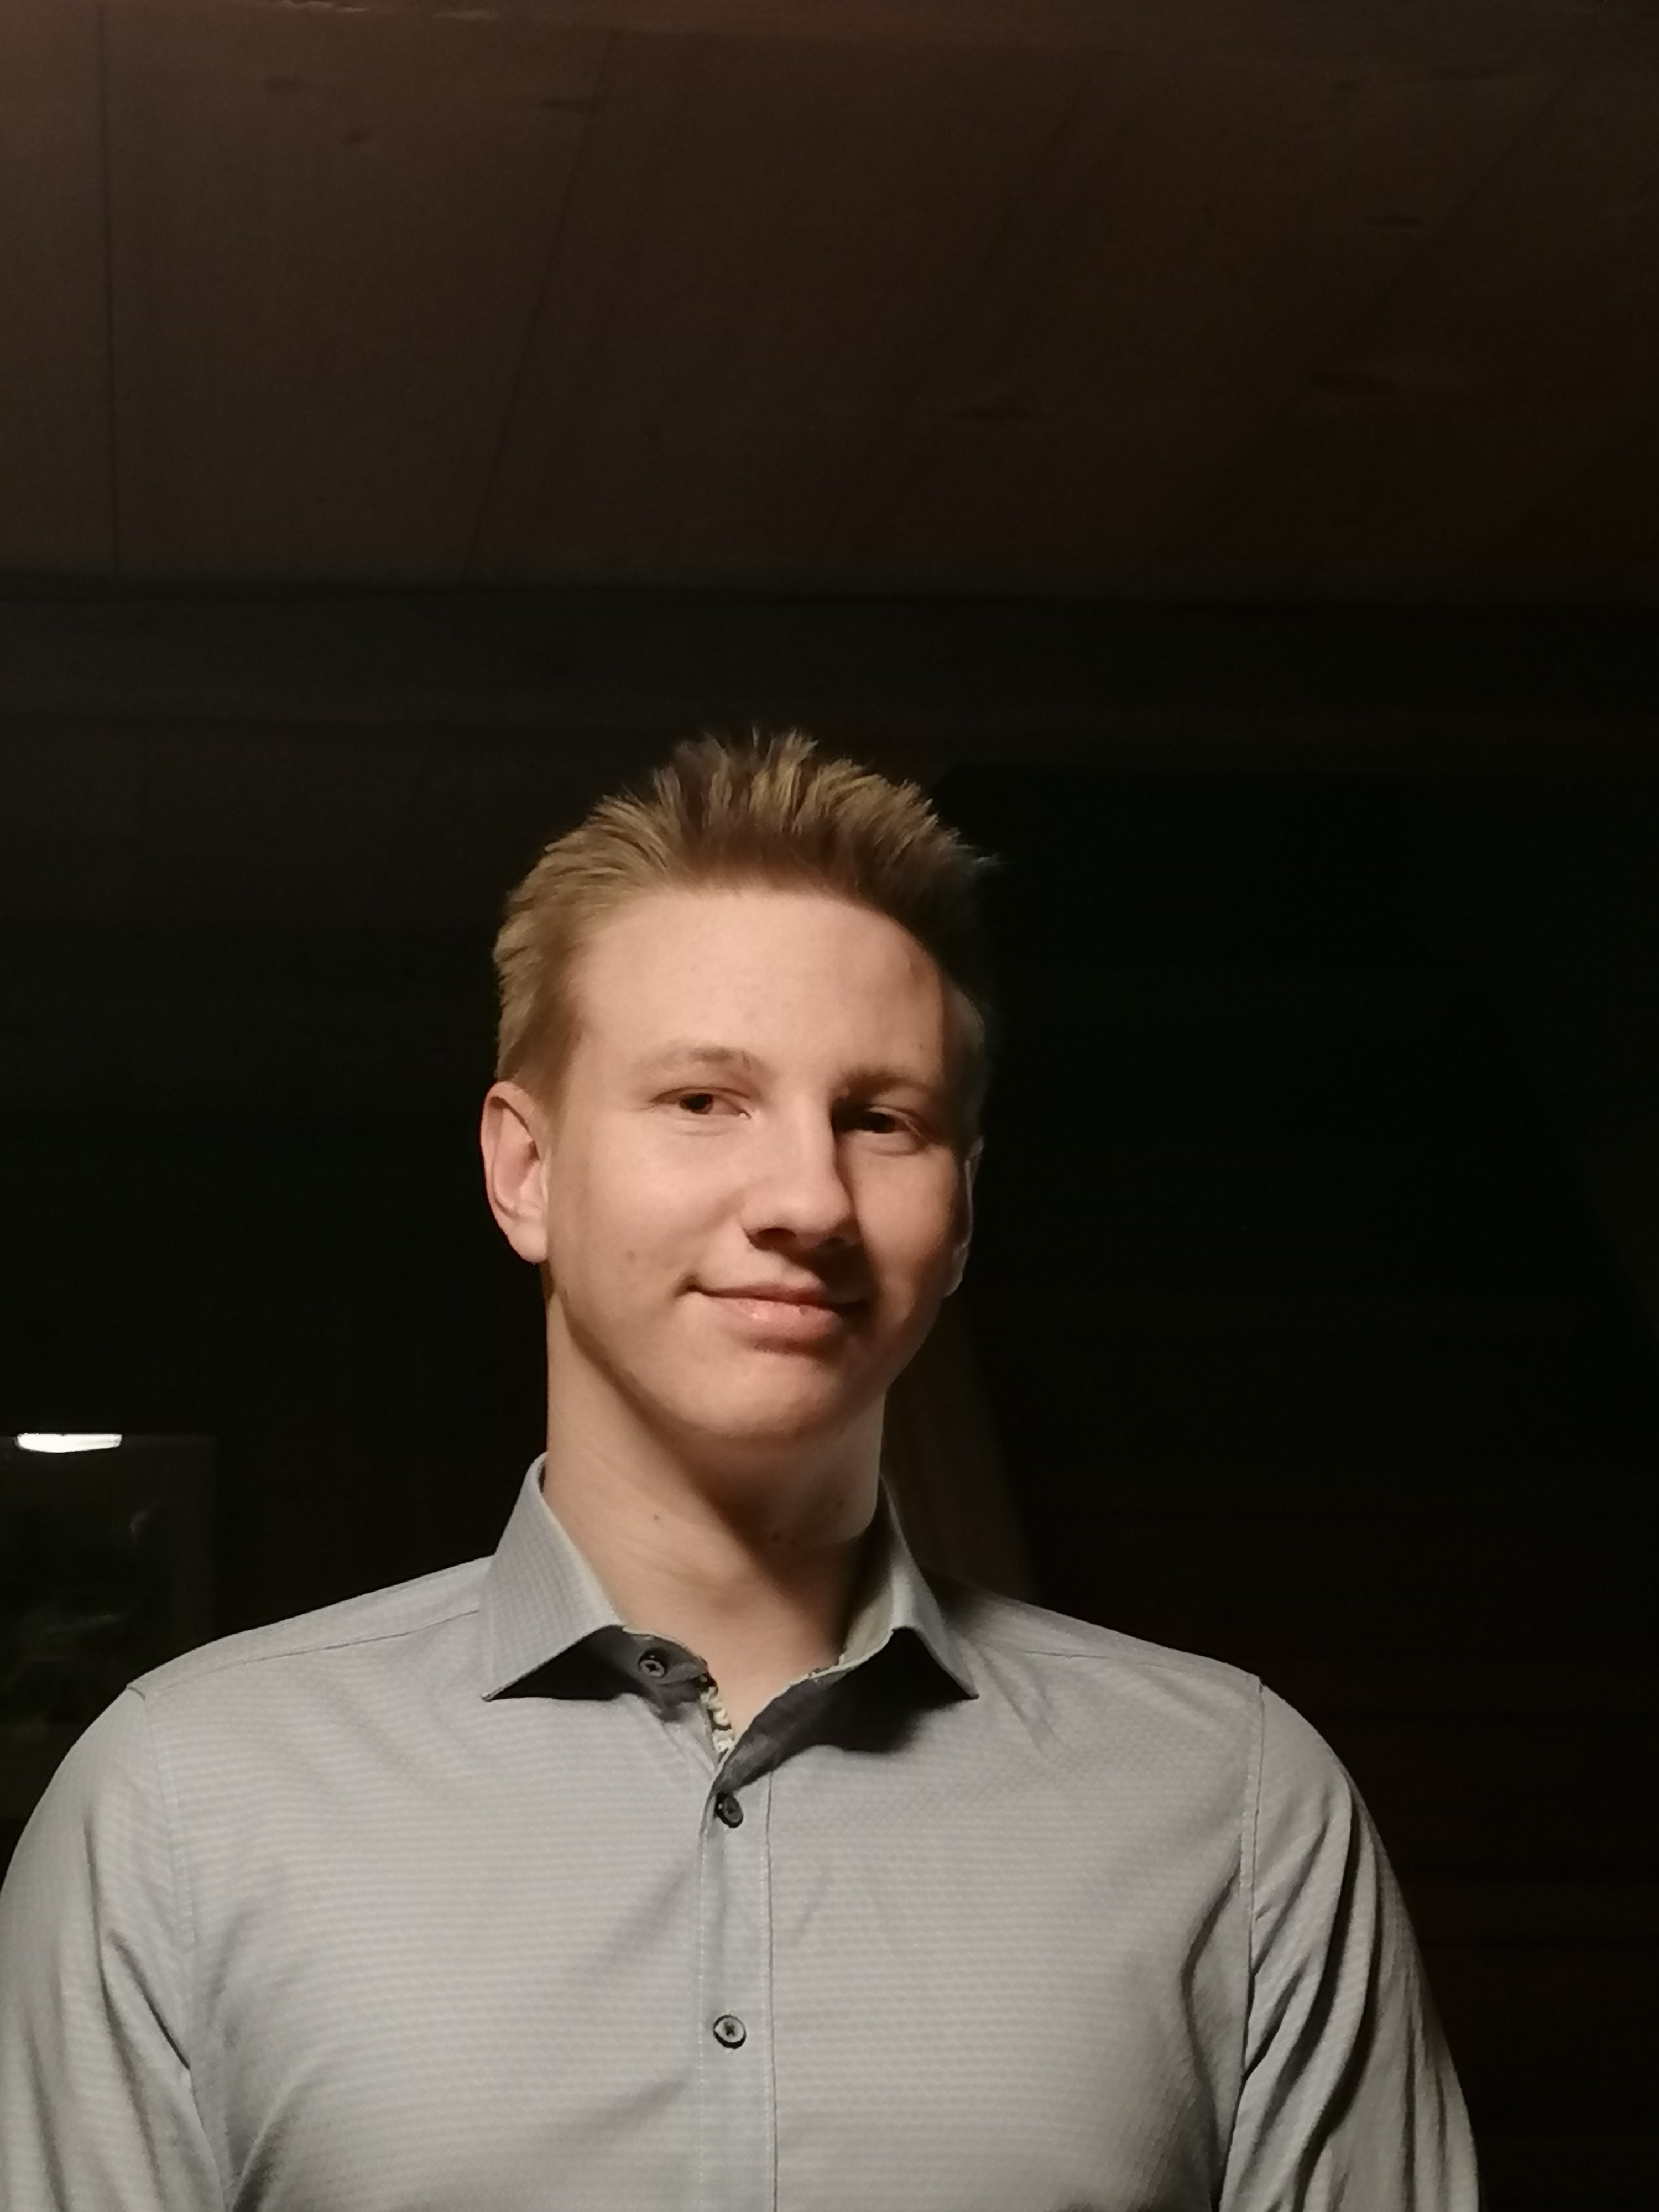
\includegraphics[width=2cm]{leo.jpg}
    &
    \vspace{0pt}
    \textbf{Leonhard Erharter} 
    \newline Adresse
    \newline PLZ Ort
    \newline
    \newline Tel: -
    \newline E-Mail: leerharter@tsn.at
    \\
\end{tabular}

\section*{Betreuer}

\begin{tabular}[t]{p{2cm} p{5cm}}
    \vspace{0pt}
    %
\includegraphics[width=2cm]{../images/betreuer.jpg}
    &
    \vspace{0pt}
    \textbf{Philipp Wischounig}
    \newline Adresse
    \newline PLZ Ort
    \newline
    \newline Tel: -
    \newline E-Mail: philipp.wischounig@htlinn.ac.at
    \\
\end{tabular} 

\newpage
\section*{Danksagung}

Am meisten danke ich meinem Betreuer, Herrn \textit{Philipp Wischounig} für die, Angesichts der widrigen Umstände, herrausragende Betreuung der Arbeit.

Weiters danke ich Herrn \textit{Lukas Fenz} für Seine Expertise im Gebiet der Elektronik, sowie den Herren \textit{Joshua Winkler} und \textit{Nicolaus B. Rossi} für Ihre Hilfsbereitschaft beim Korrekturlesen der Arbeit.

Zuletzt danke ich meiner Familie für die mentale Unterstützung, Motivation, sowie die Bereitstellung der für die Durchführung nötigen Werkzeugen.

\newpage
\section*{Gendererklärung}

Aus Gründen der besseren Lesbarkeit wird in dieser Diplomarbeit durchweg die Sprachform des generischen Maskulinums angewendet. An dieser Stelle wird darauf hingewiesen, dass die ausschließliche Verwendung der männlichen Sprachform geschlechtsunabhängig verstanden werden soll.

\newpage
\section*{Abstract}

Insert English abstract here

...

\newpage
\section*{Zusammenfassung}

Das Thema Elektromotoren ist ein umfangreicher und komplexer Teil des Unterrichts, welchen die Schüler erlernen müssen. Die dafür benötigte Zeit wird durch das Fehlen adäquater Unterrichtsmittel, welche das Verständnis der Funktionsweise erleichtern, unnötig verlängert.

Ziel dieser Diplomarbeit ist es, neue Mittel zu schaffen, sowie bereits bestehende zu dokumentieren. Dies ermöglicht es Lehrern aus einem breiteren Spektrum benutzerfreundlicher Tools jene auszuwählen welche die Effizienz des Unterrichts steigern.

Das Ergebnis ist ein schnellerer und mitreißender Lernprozess, der dem Lehrer mehr Zeit zur Verfügung stellt um andere Punkte seines Unterrichts zu vertiefen.

\newpage
\tableofcontents
\newpage
\part{Intro}
\chapter{Hintergrund}
\input{parts/1-intro/0-hintergrund/0-allgemein.tex}
\input{parts/1-intro/0-hintergrund/1-ziel.tex}
\chapter{Situation}
\input{parts/1-intro/1-situation/0-allgemein.tex}
\input{parts/1-intro/1-situation/1-covid.tex}
\input{parts/1-intro/1-situation/2-team.tex}

\part{Theoretische Grundlagen}
\chapter{Elektromotoren}

Elektromotoren sind heutzutage in beinahe allen Bereichen des Lebens aufzufinden. 
Ihre größten Unterschiede zu konventionellen Verbrennungsmotoren sind:
\begin{itemize}
    \item höherer Wirkungsgrad
    \item meistens geringere Wartungs- sowie Produktionskosten
    \item leiser als Verbrennungsmotoren
\end{itemize}

In den folgenden individuellen Betrachtungen der gängigsten Arten werden diese als "Maschinen" bezeichnet.
Der Hintergrund hierfür ist, dass diese entweder mit geringfügigen oder ganz ohne Veränderungen als Generatoren betrieben werden können.

Da die Funktion als Generator im Zuge dieser Arbeit nicht von Bedeutung ist, wird nachfolgend nur die Funktion als Motor eingehend erläutert.

\section{Gleichstrommaschinen}
\input{parts/2-theorie/0-dc-motoren/0-allgemein.tex}
\input{parts/2-theorie/0-dc-motoren/1-perma.tex}
\input{parts/2-theorie/0-dc-motoren/2-fremd.tex}
\input{parts/2-theorie/0-dc-motoren/3-reihen.tex}
\input{parts/2-theorie/0-dc-motoren/4-neben.tex}

\chapter{Wechselstrommaschinen}
\input{parts/2-theorie/1-ac-motoren/0-allgemein.tex}
\input{parts/2-theorie/1-ac-motoren/1-asynchron.tex}
\input{parts/2-theorie/1-ac-motoren/2-synchron.tex}


\part{Arbeitsmittel}
\chapter{Arbeitsbereich}
\label{arbeitsbereich}
\input{parts/3-arbeitsmittel/0-arbeitsbereich/0-allgemein.tex}
\input{parts/3-arbeitsmittel/0-arbeitsbereich/1-anforderungen.tex}
\input{parts/3-arbeitsmittel/0-arbeitsbereich/2-design.tex}
\input{parts/3-arbeitsmittel/0-arbeitsbereich/3-auswahl.tex}
\input{parts/3-arbeitsmittel/0-arbeitsbereich/4-endprodukt.tex}
\part{Appendix}
\input{parts/8-appendix/0-zeitaufwand.tex}
\chapter{Bauteile}
\input{parts/3-arbeitsmittel/2-bauteile/0-allgemein.tex}
\input{parts/3-arbeitsmittel/2-bauteile/1-bauteile.tex}
\chapter{Software}
\input{parts/3-arbeitsmittel/3-software/0-allgemein.tex}
\input{parts/3-arbeitsmittel/3-software/1-software.tex}

\part{Vorzeigemodell}
\chapter{Gleichstrommaschine}
\section{Anleitung}

Der gegebene Aufbau kann durch spezifische Verkabelung entweder als \hyperref[neben]{\textit{Nebenschlussmaschine}}, oder als \hyperref[reihen]{\textit{Reihenschlussmaschine}} verwendet werden.

Bei Vorhandensein von zwei Spannungsquellen ist auch die Verwendung als \hyperref[fremd]{\textit{fremderregte}} Gleichstrommaschine möglich, dies wird hier jedoch nicht dokumentiert.

\subsection{Nebenschlussschaltung}

Um den Aufbau als Nebenschlussmaschine zu schalten müssen sowohl die Spulen, als auch die Schleifer parallel geschalten werden wie auf folgendem Bild.

\begin{figure}[H]
    \centering
    \hfill
    \subfigure[Foto Nebenschlussschaltung]{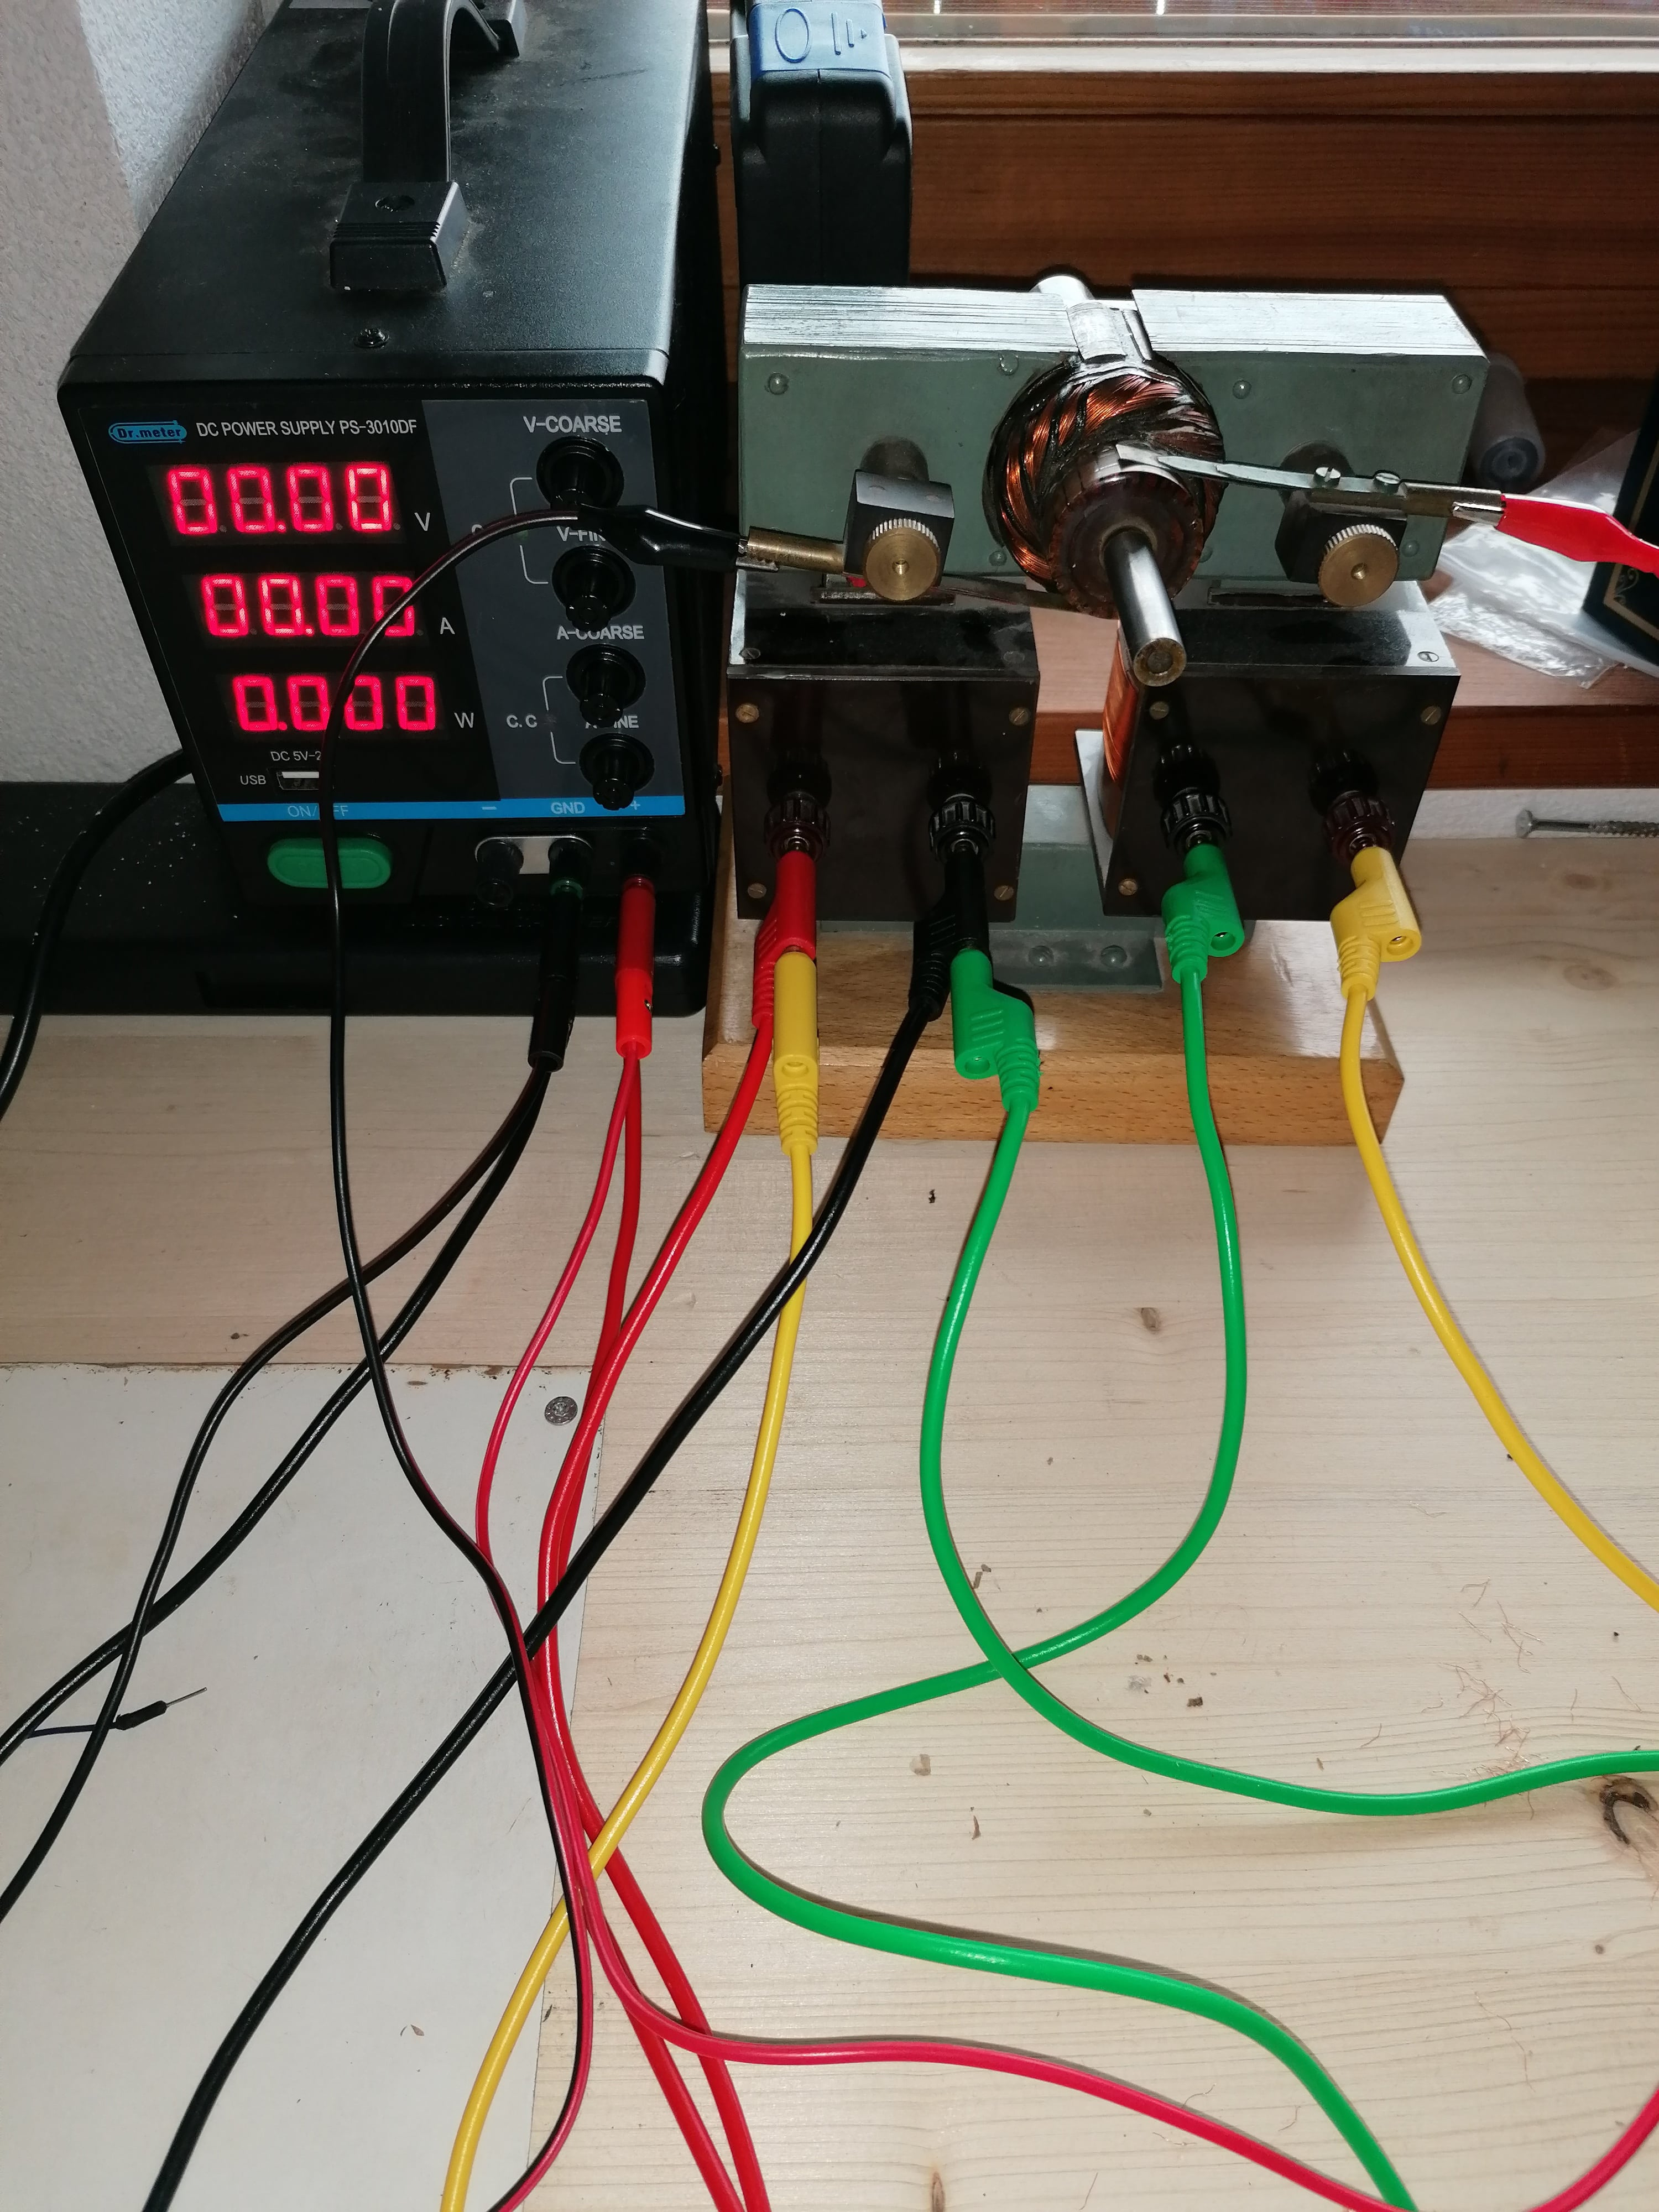
\includegraphics[width=0.3\textwidth]{nebenschluss.jpg}}
    \hfill
    \subfigure[Nebenschlussmaschine laut Wikipedia ~ \cite{wikipedia:neben}]{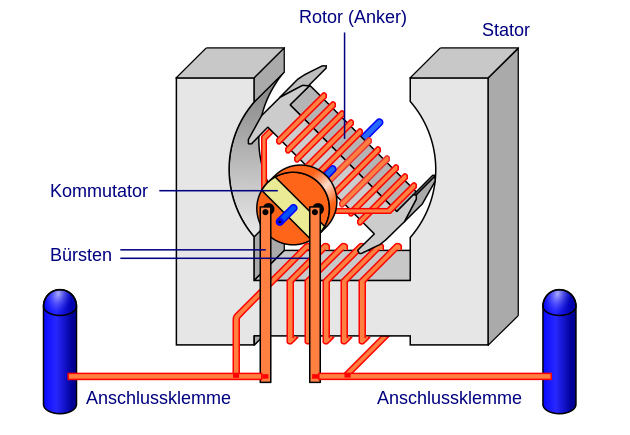
\includegraphics[width=0.3\textwidth]{nebenschlusswiki.png}}
    \hfill
    \caption{Nebenschlussschaltung in 2 Erklärungen}
\end{figure}

Um die Funktionsweise einer Nebenschlussmaschine zu beweisen können die beiden Verbindungen zu den Schleifern vertauscht werden, was die Drehrichtung umkehrt.

\subsection{Reihenschlussschaltung}

Um den Aufbau als Hauptschlussmaschine zu schalten müssen beide Schaltkreise in Reihe geschalten werden.
Das bedeutet, dass der positive Ausgang der Spannungsversorgung nur direkt mit einem der beiden Schleifer oder den Spulen verbunden werden darf.
Für den negativen Ausgang gilt das Gleiche.

\begin{figure}[H]
    \centering
    \hfill
    \subfigure[Foto Reihenschlussschaltung]{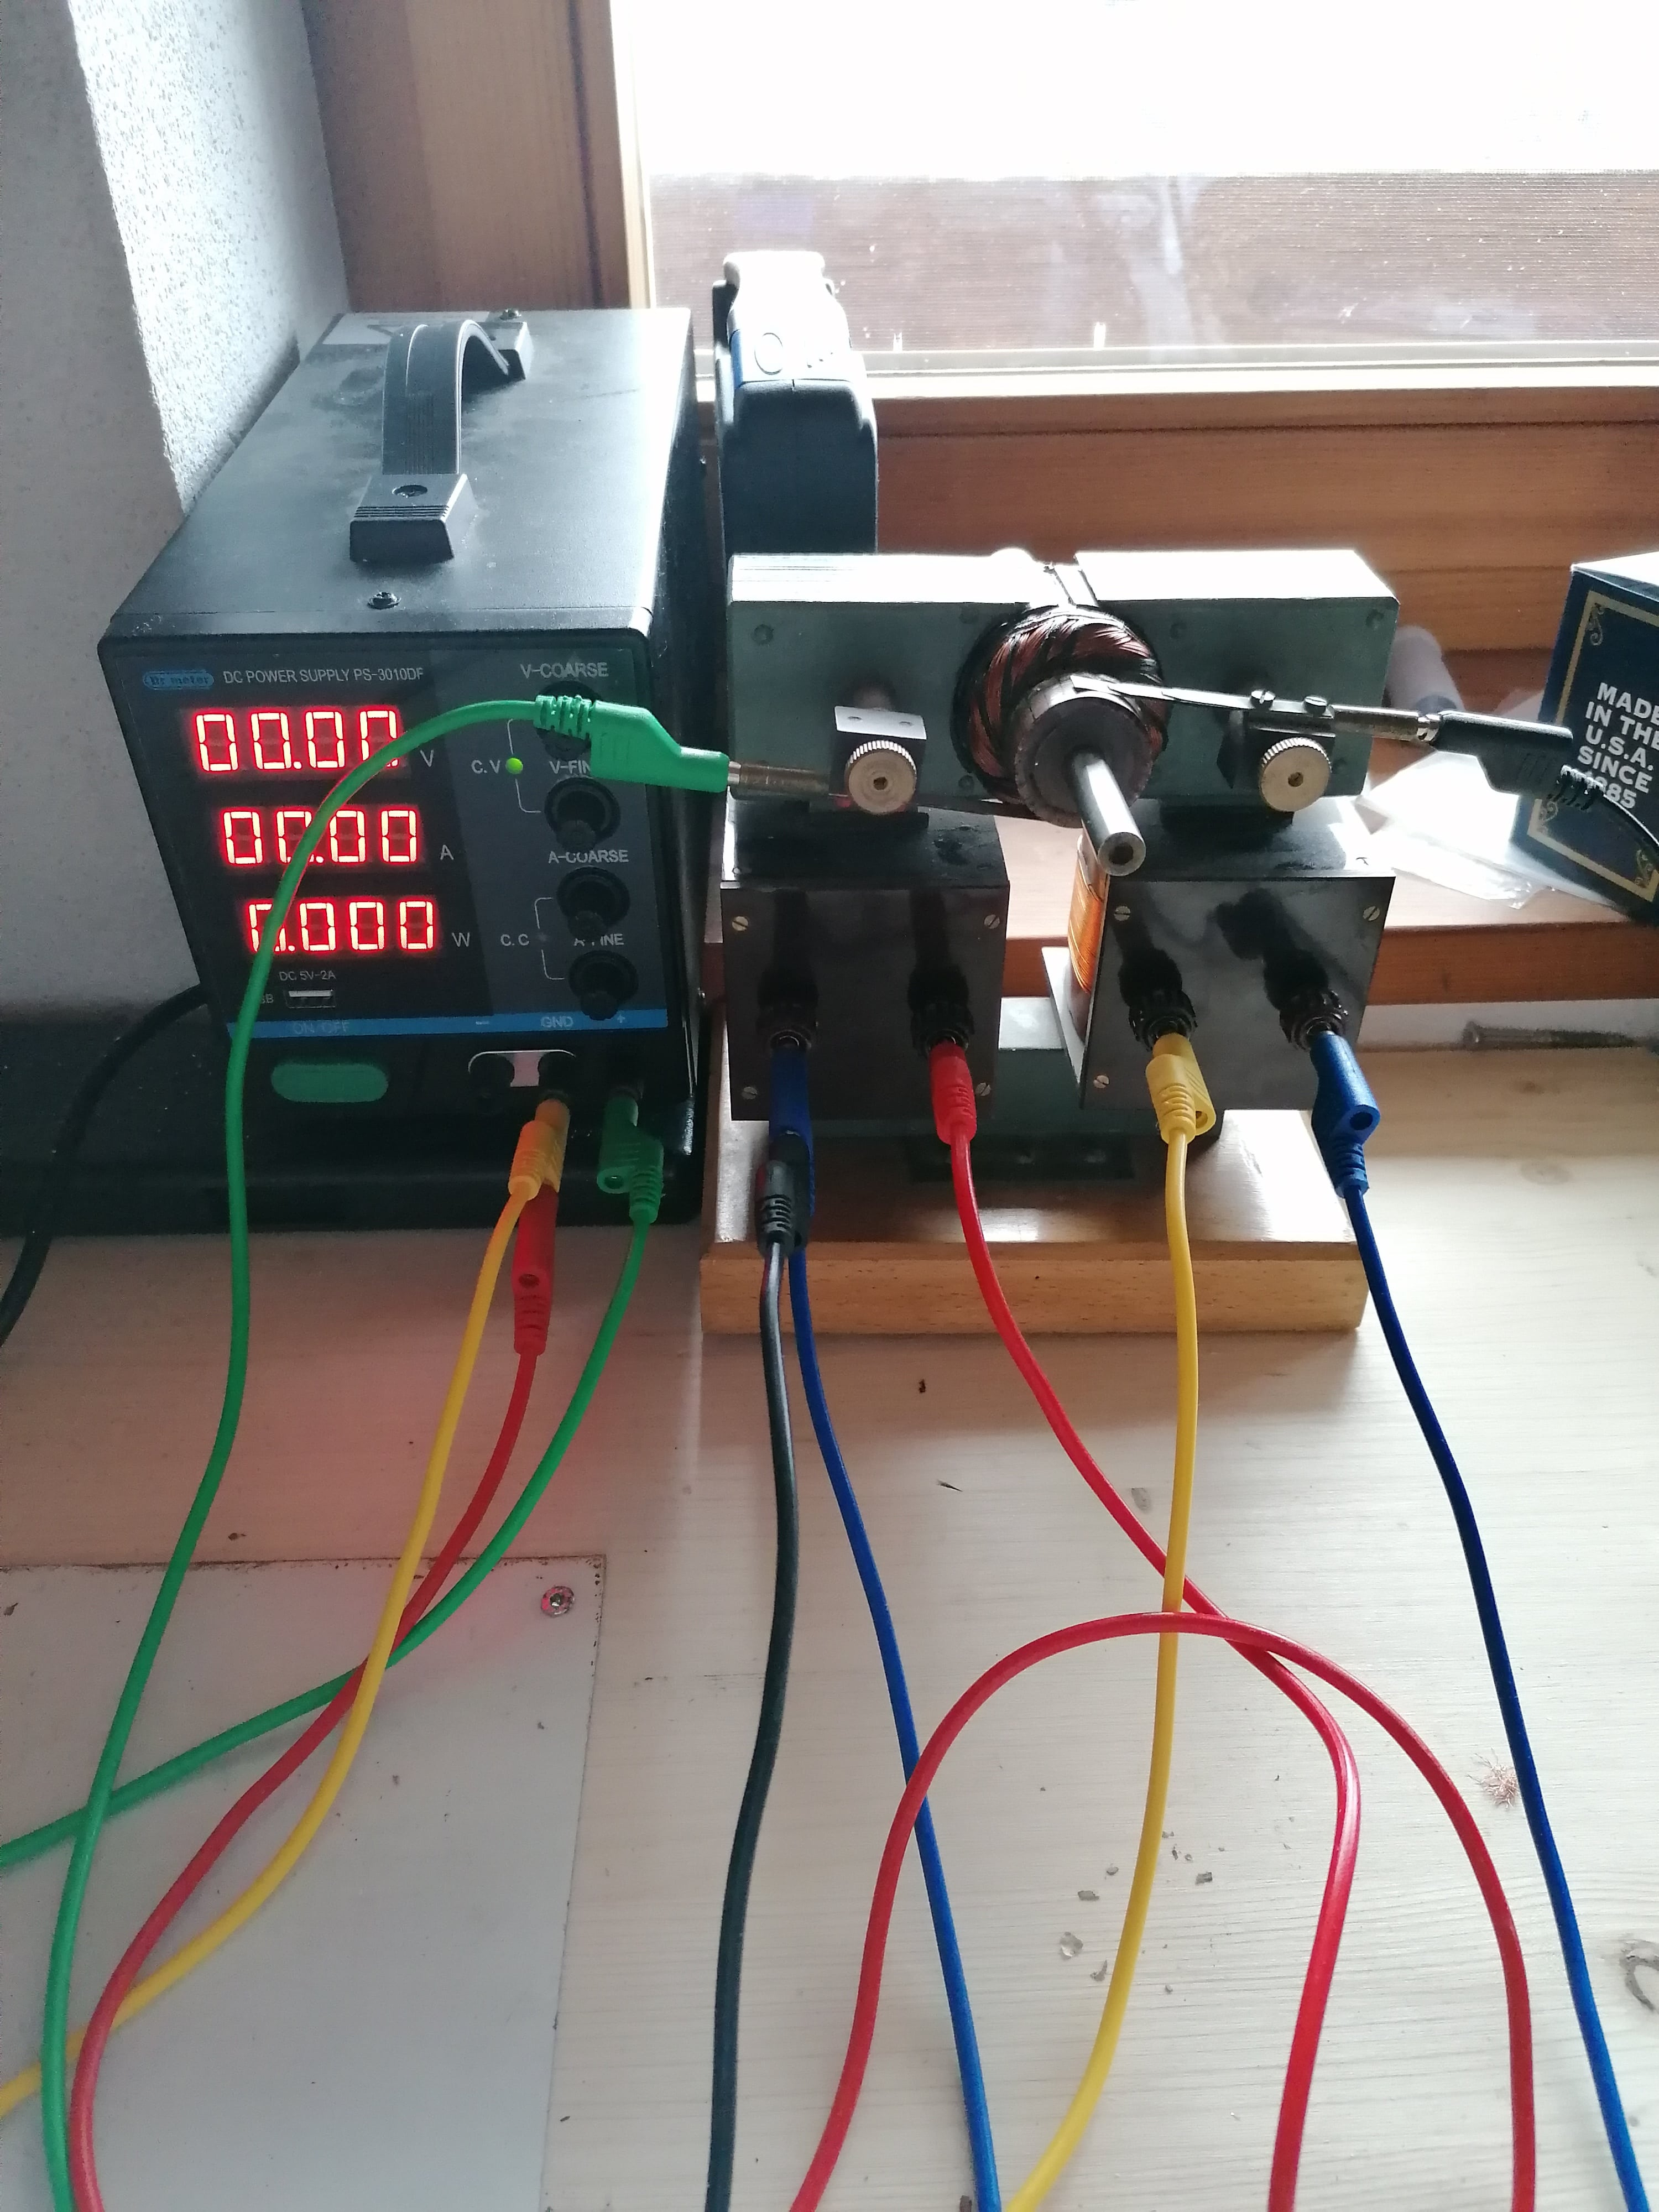
\includegraphics[width=0.3\textwidth]{hauptschluss.jpg}}
    \hfill
    \subfigure[Reihenschlussmaschine laut Wikipedia ~ \cite{wikipedia:reihen}]{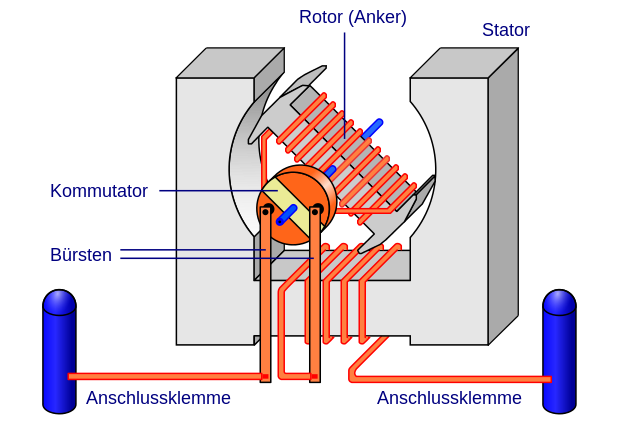
\includegraphics[width=0.3\textwidth]{reihenschlusswiki.png}}
    \hfill
    \caption{Reihenschlussschaltung in 2 Erklärungen}
\end{figure}

Hier kann bewiesen werden, dass bei Vertauschen der Verbindungen zu den Schleifern die Drehrichtung gleich bleibt.
\input{parts/4-vorzeigemodell/2-vorschläge.tex}
\part{Versuchsaufbau}
\chapter{Ziel des Aufbaues}

Durch den Versuchsaufbau soll es möglich sein die Motorkennlinie eines Elektromotors nachzuweisen.
Hierfür muss

\begin{itemize}
    \item die Drehzahl gemessen,
    \item sowie durch Bremsen des Motors das Drehmoment ermittelt werden.
\end{itemize}

Weiters soll der Aufbau zur Durchführung einer Laborübung wie unter  \hyperref[labuebung]{Teil 6} verwendet werden.
\chapter{Anforderungen}
\input{parts/5-versuchsaufbau/0-anforderungen/0-allgemein.tex}
\input{parts/5-versuchsaufbau/0-anforderungen/1-drehzahl.tex}
\input{parts/5-versuchsaufbau/0-anforderungen/2-drehmoment.tex}
\input{parts/5-versuchsaufbau/0-anforderungen/3-bremse.tex}
\chapter{Versionen}
\input{parts/5-versuchsaufbau/1-versionen/0-allgemein.tex}
\input{parts/5-versuchsaufbau/1-versionen/1-provisorium.tex}
\input{parts/5-versuchsaufbau/1-versionen/2-laborform.tex}

\chapter{Finalisierung}
\input{parts/5-versuchsaufbau/2-finalisierung/0-allgemein.tex}
\input{parts/5-versuchsaufbau/2-finalisierung/1-gegenkupplung.tex}
\input{parts/5-versuchsaufbau/2-finalisierung/2-drehzahlmessung.tex}
\input{parts/5-versuchsaufbau/2-finalisierung/3-rohrschelle.tex}
\part{Laboruebung}
\chapter{Anforderungen}

Die zum Versuchsaufbau entworfene Laborübung soll folgende Anforderungen erfüllen.

\begin{itemize}
    \item verständlich verfasst
    \item Interesse weckend
    \item Eigeninitiative fördernd
\end{itemize}
\chapter{Laborübung}

\section{Erstellung}

Die Laborübung wurde mit Microsoft Word verfasst, da zum Zeitpunkt der Erstellung noch nicht feststand, dass die Verschriftlichung der Arbeit in LaTeX erfolgen würde.

Aufgrund dessen weicht die Formatierung auf den folgenden Seiten vom Rest des Dokumentes ab.

\section{Anforderungen}

Die zum Versuchsaufbau entworfene Laborübung soll folgende Anforderungen erfüllen.

\begin{itemize}
    \item verständlich verfasst
    \item Interesse weckend
    \item Eigeninitiative fördernd
\end{itemize}

Die Altersgruppe für welche diese Übung geschaffen wurde dürfte bereits Erfahrungen mit der Arbeit mit Arduinos haben.
Die Struktur des Laborberichtes ist abhängig vom Pädagogen, welcher diese Übung beaufsichtigt, weshalb nur auf die gewünschten Inhalte eingegangen wird.

\section{Laborübung}

\label{labuebung}
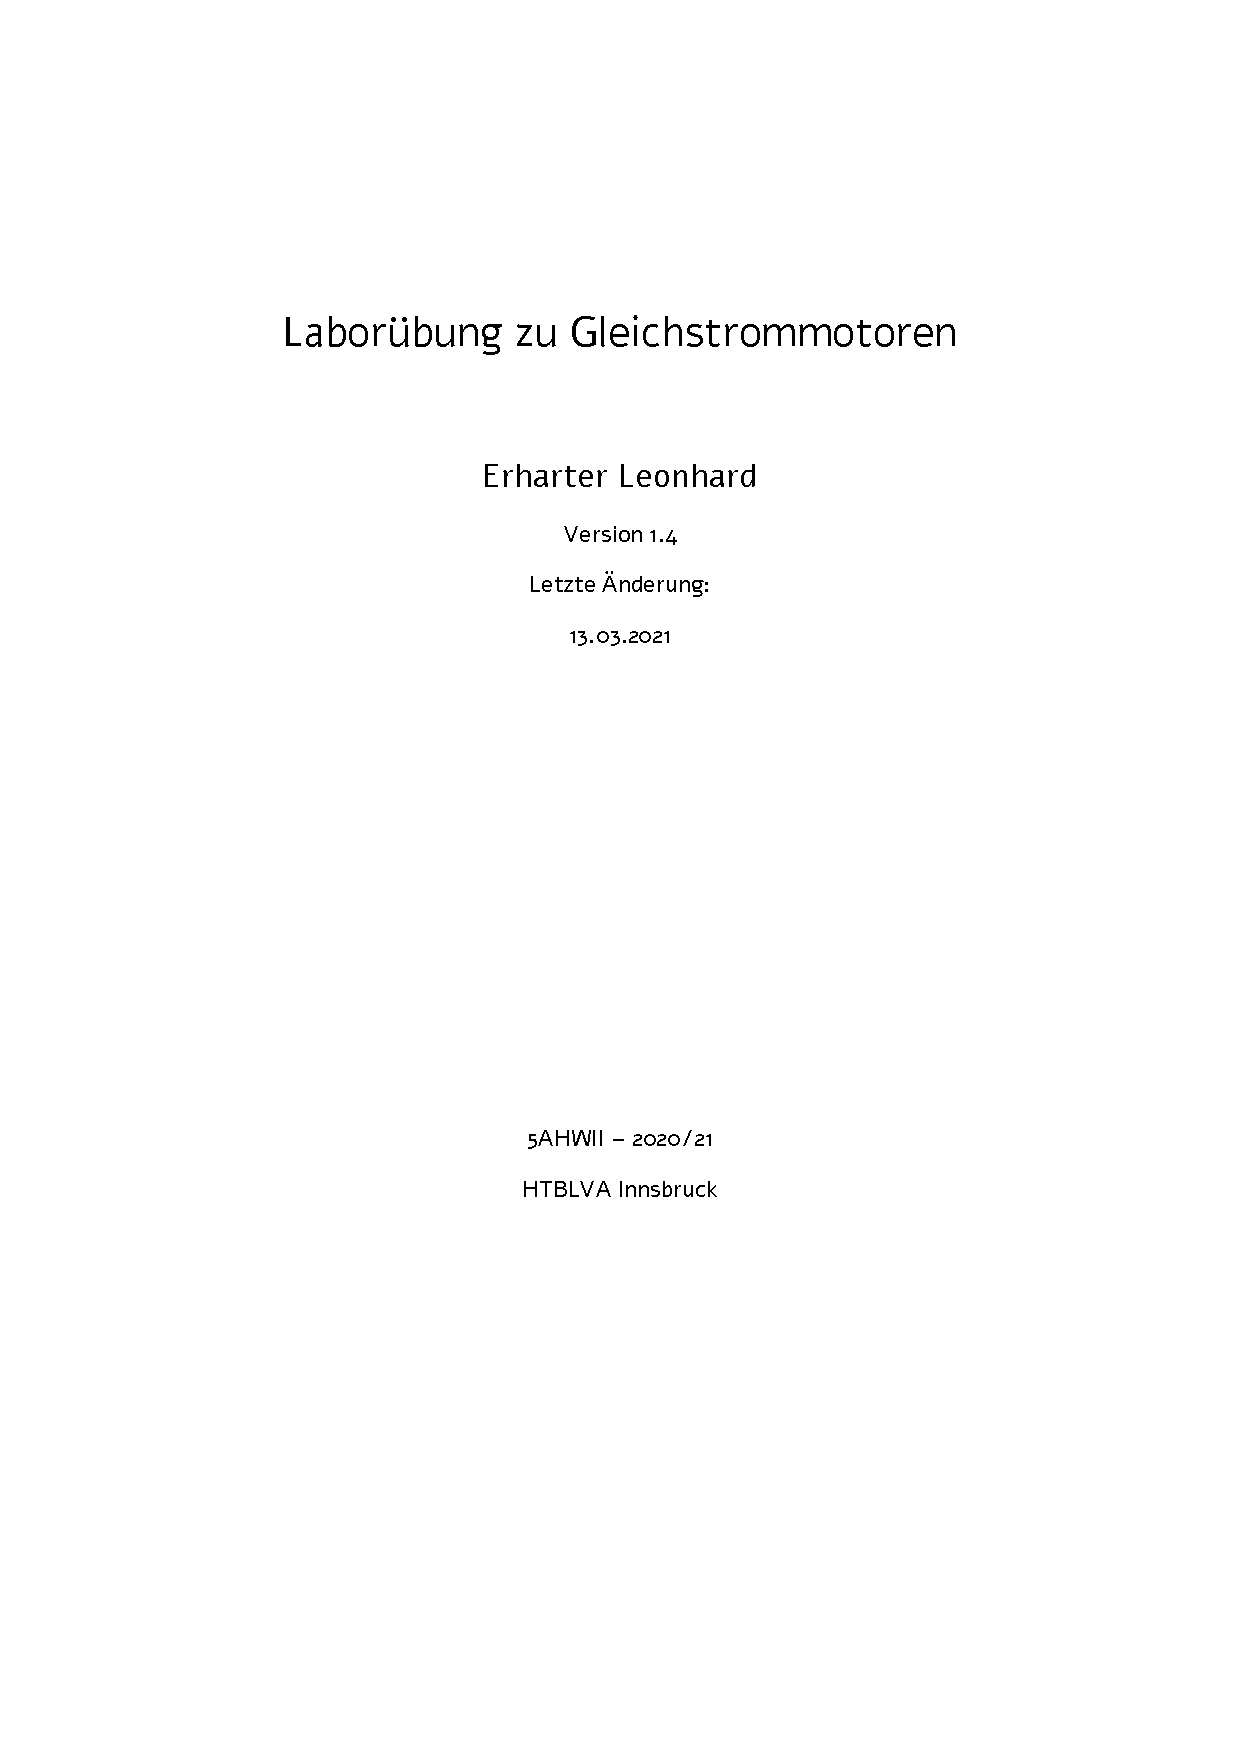
\includepdf[pages=-]{files/LaboruebungV04.pdf}
\chapter{Musterlösung}

\label{muster}
Die Musterlösung wurde mit dem Online Markdown Editor Hedgedoc verfasst, was im Falle von Laborteams eine mühelose Zusammenarbeit ermöglicht.
Somit differenziert sich auch auf den folgenden Seiten die Struktur des Dokumentes von der restlichen Dokumentation der Arbeit.

Da zum Zeitpunkt der Verfassung dieses Dokuments nur ein provisorischer Versuchsaufbau zur Durchführung der Aufgaben bereit stand, war es im Zuge dieser Musterlösung nicht möglich Probleme welche exklusiv bei Verwendung des laborfertigen Versuchsaufbaues entstehen könnten zu simulieren.
Jedoch sind diese Unterschiede nur gering, weshalb dieses Muster auch bei Verwendung des laborfertigen Versuchsaufbaues Relevanz hat.

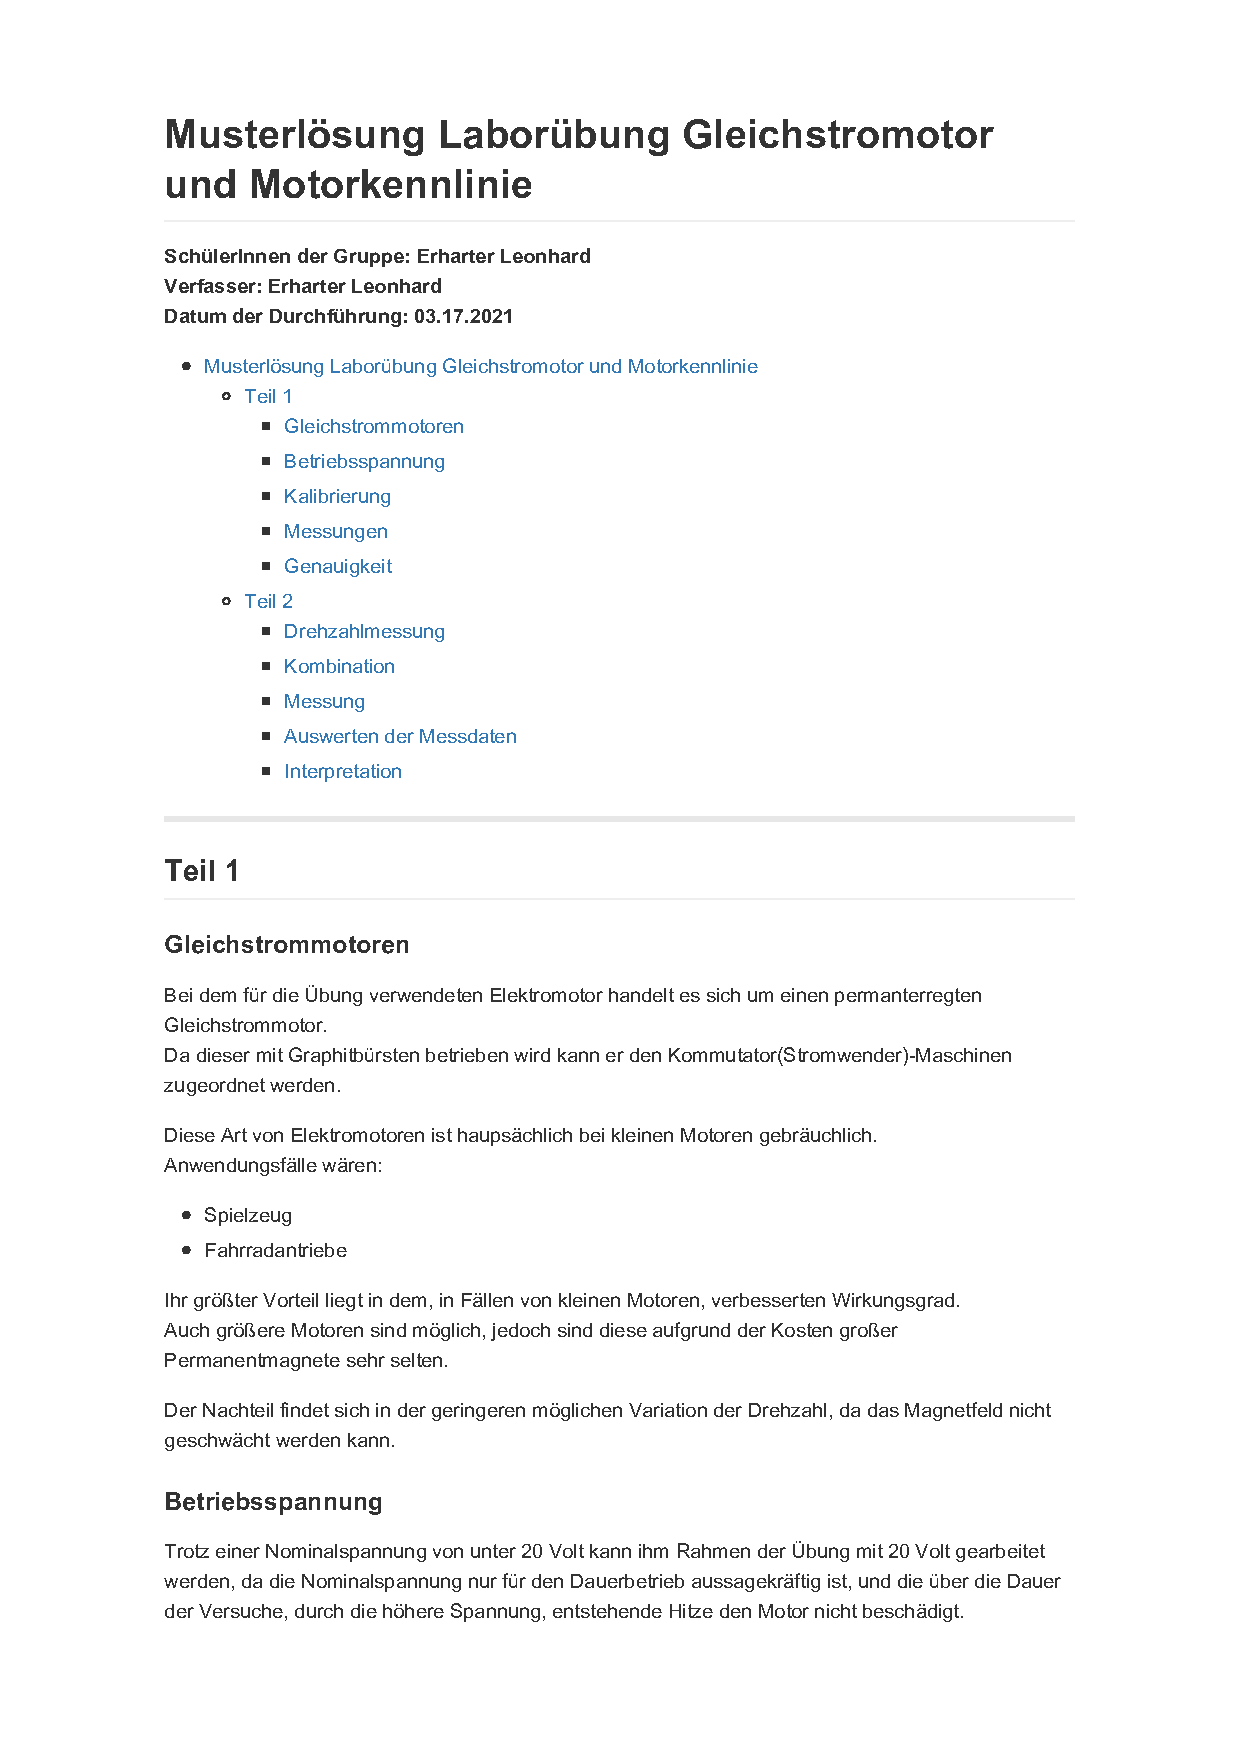
\includepdf[pages=-]{files/Muster.pdf}
\part{Rückblick}
\chapter{Rückblick auf den Verlauf}

Im Rückblick werden Probleme bei der Organisation der Arbeit genauer untersucht.
\section{Aufgabenteilung}

Bei der Aufgabenteilung konnte durch die konkrete Projektsituation bemerkt werden, dass eine noch individuellere Abgrenzung der Aufgaben sinnvoll gewesen wäre.

Dies hätte das Durchführen als Einzelarbeit erleichtert, da so in keinem Falle Abhängigkeit vom Teampartner bestünde.
\chapter{Kommunikation}
\part{Appendix}
\addcontentsline{toc}{chapter}{Zeitaufwand}
\chapter*{Zeitaufwand}

TODO: Zeitaufwand digitalisieren und einfügen
\setcounter{secnumdepth}{1}
\appendix

\cleardoublepage
\phantomsection
\addcontentsline{toc}{chapter}{Literaturverzeichnis}
\bibliography{references} %references bibtech as used for all papers dealing with online-surveys
\nocite{*}

\cleardoublepage
\phantomsection
\addcontentsline{toc}{chapter}{\listfigurename}
\listoffigures
\cleardoublepage
\phantomsection
\addcontentsline{toc}{chapter}{Code-Snippet-Verzeichnis}
\listof{code}{Code-Snippet-Verzeichnis}

\end{document}